\section{Detaljert arkitektur} %TODO denne må splittes og flyttes.
\label{sec:arkitektur}
Presentasjon av varsling opp til førerhus, implementeres som MVC-pattern, 
hvor den sentrale prosesseringsenheten har controller-rollen og gjør alle 
de sentrale utregningene for systemet. Controlleren sender de prosesserte 
dataene til viewet, som i denne sammenhengen er smartskjermen plassert i 
dashbordet. Ved utvidelse til støtte for rapportering av spesifikke, 
kjente feil, implementeres modelstøtte i prosesseringsenheten som en 
``database'' av tupler bestående av signal og tilhørende feilmelding. 

Sammenhengen mellom modellen, viewet og controlleren ses i figur \ref{fig:mvc}.
\newline
\begin{figure}[H]
	\centering
	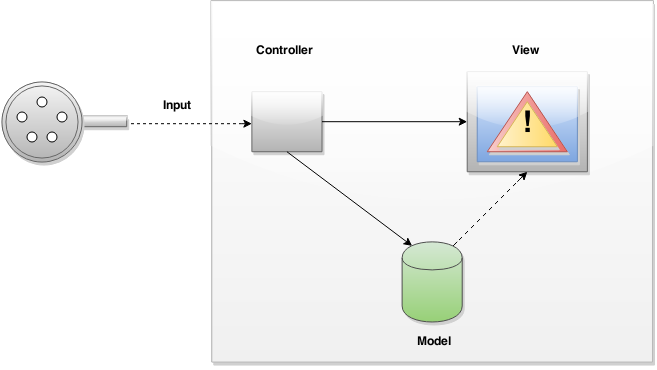
\includegraphics[width=1.00\textwidth]{images/architecture2-mvc.png}
	\label{fig:mvc}
	\caption{Arkitekturskisse: Model view controller.}
\end{figure}